\documentclass[10pt, aspectratio=169]{beamer}
\usepackage{caption}
\usepackage{subcaption}
\usetheme[progressbar=frametitle]{metropolis}
\usepackage{amsmath}
\usepackage{siunitx}
\usepackage{xcolor}
\usecolortheme{crane}
\definecolor{craneorange}{rgb}{0.53,0.66,0.42}
\usecolortheme{spruce}
\usepackage{hyperref}
\usepackage{multimedia}
\usepackage[percent]{overpic}
\usepackage[para]{footmisc}

\title{Computational study of far-field acoustic emission by collapsing bubbles}
\date{\today}
\author[shortname]{Magu Raam Prasaad R}
\institute[shortinst]{Indian Institute of Science, Bangalore}

\begin{document}

\begin{frame}
	\maketitle
\end{frame}

\begin{frame}{Introduction}
	\begin{columns}
		\column{0.5\textwidth}
		\begin{itemize}
			\item High-speed flows lead to the formation of cavitation bubbles.
			\item Collapsing cavitation bubbles form blast and shock waves.
			\item Blastwave emission processes are a strong source of acoustic waves.
			\item Bubbles strongly interact with and produce sound.
		\end{itemize}
				
		\column{0.5\textwidth}
		\begin{figure}[h]
			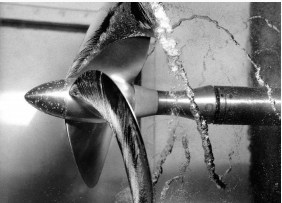
\includegraphics[scale = 0.55]{images/propeller.png}
			\caption*{Cavitation bubbles around rotating propeller\cite{propeller}}	
		\end{figure}
							
	\end{columns}
	\footnotetext[1]{Brennen C. E, JFM 2002}
\end{frame}

\begin{frame}{Objective}
	\begin{columns}
		\column{0.5\textwidth}

	\begin{itemize}
		\item To simulate the single and multiple cavitation bubble collapse processes.
		\item Compute the far-field acoustic waves emitted by collapsing bubbles using the Boundary integral method.
		\item To analyze the acoustic wave generation and propagation.
	\end{itemize}
				
		\column{0.5\textwidth}
		\begin{figure}[h]
			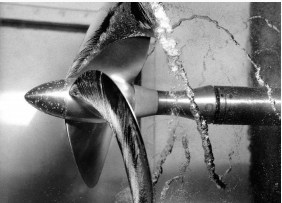
\includegraphics[scale = 0.55]{images/propeller.png}
			\caption*{Cavitation bubbles around rotating propeller\cite{propeller}}	
		\end{figure}
							
	\end{columns}
	\footnotetext[1]{Brennen C. E, JFM 2002}
\end{frame}

\begin{frame}{Computational approach}
	
	\begin{itemize}
		\item Compute the far-field acoustic waves emitted from the bubble collapse process using the Kirchhoff integral formulation.
	\end{itemize}

	\begin{figure}
		\centering
		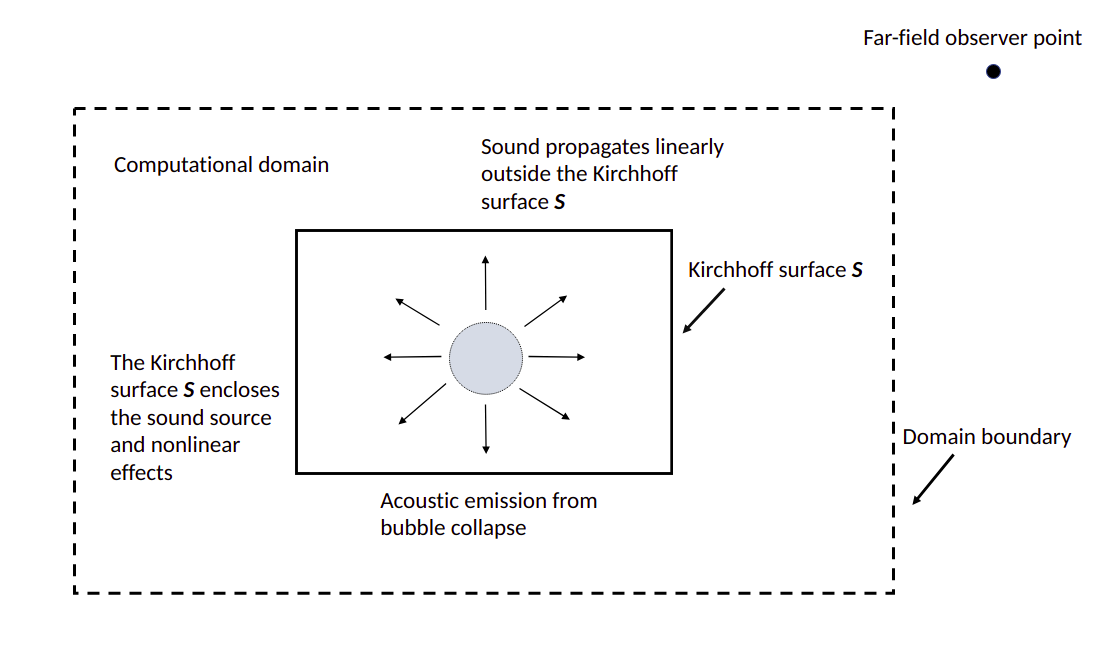
\includegraphics[scale=0.22]{images/shematic1.png}
		\caption*{Schematic of far-field acoustic data computed from CFD solver using the Kirchhoff integral method.}
	\end{figure}		

\end{frame}

\begin{frame}{Kirchhoff integral formulation}
	\begin{columns}
		\column{0.5\textwidth}
		\begin{itemize}
			\item We chose a control surface $S$ that encloses all the acoustic sources, and the pressure perturbations $p'$ satisfies the homogeneous wave equation.
			\begin{equation}\label{Wave equation}
				\Bigg( \frac{1}{c_{0}^2}\frac{\partial{}^{2}}{\partial{t}^{2}}- \nabla{}^{2} \Bigg) p' = 0 \quad \quad \textrm{in} \ V.
			\end{equation}
			\item The control surface S is defined by $f(\mathbf{x}) = 0$, $f(\mathbf{x}) > 0$ for $\mathbf{x}$ in V and $f(\mathbf{x}) < 0$ for $\mathbf{x}$ inside surface S.
		\end{itemize}
				
		\column{0.5\textwidth}
		\begin{figure}[h]
			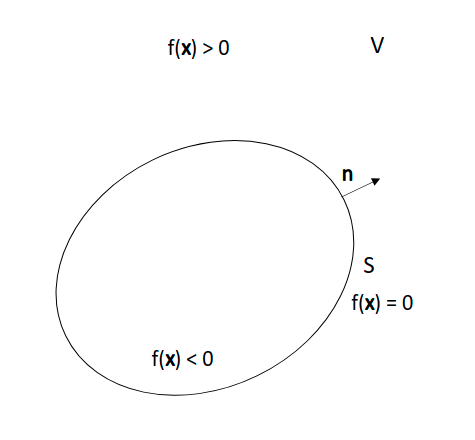
\includegraphics[scale = 0.3]{images/kirchhoff_surface.png}
			\caption*{Stationary Kirchhoff surface $S$ encloses sound source}	
		\end{figure}
							
	\end{columns}
\end{frame}

\begin{frame}{Kirchhoff integral formulation}
	\begin{columns}
		\column{0.5\textwidth}
		\begin{itemize}
			\item We define the pressure $p'$ as a generalized function $pH(f)$ where
			\begin{equation*}\label{Generalized_Functions}
				p' H(f) =\begin{cases}
					p' , & \text{for $\mathbf{x}$ in V}.     \\
					0,  & \text{for $\mathbf{x}$ inside S}.
				\end{cases}
			\end{equation*}
			\item The acoustic wave equation in generalised pressure
			\begin{equation*}\label{Generalized Wave Equation}
				\Bigg( \frac{1}{c_{0}^2}\frac{\partial{}^{2}}{\partial{t}^{2}}- \nabla{}^{2} \Bigg) p'H = -\frac{\partial p'}{\partial n}\delta(f) - \nabla.(p' \mathbf{n} \delta(f)).
			\end{equation*}
		\end{itemize}
				
		\column{0.5\textwidth}
		\begin{figure}[h]
			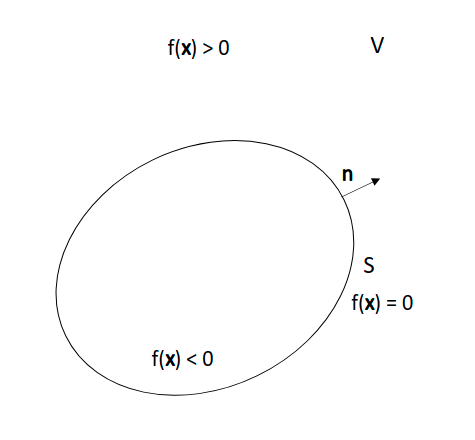
\includegraphics[scale = 0.3]{images/kirchhoff_surface.png}
			\caption*{Stationary Kirchhoff surface $S$ encloses sound source}	
		\end{figure}
							
	\end{columns}
\end{frame}

\begin{frame}{Kirchhoff integral formulation}
	\begin{itemize}
		\item The acoustic wave equation in generalized variables is valid in the
		entire unbounded space. Therefore we can use the free-space Green’s function to
		solve the equation.
		\begin{equation}\label{pressure}
			p'(\mathbf{x}, t) = \int s(\mathbf{y}, \tau){G(\mathbf{x}, t; \mathbf{y}, \tau )} d\mathbf{y}d\tau.
		\end{equation}
		where,
		\begin{equation}\label{Green's Function}
			G(\mathbf{x}, t; \mathbf{y}, \tau ) = \frac{\delta \Big(t - \tau - \frac{|\mathbf{x} - \mathbf{y}|}{c_{0}}\Big)}{4\pi|\mathbf{x} - \mathbf{y}|}
		\end{equation}
		and 
		\begin{equation}
			s(\mathbf{y}, \tau) = -\frac{\partial p'}{\partial n}\delta(f) - \nabla.(p' \mathbf{n} \delta(f)).
		\end{equation}
	\end{itemize}
\end{frame}

\begin{frame}{Kirchhoff integral formulation}
	\begin{itemize}
		\item The Kirchhoff integral equation for a stationary control surface is given by
		      \begin{equation}
			      \begin{split}
				      p'(\mathbf{x}, t) = \frac{1}{4\pi}\int_{S}\Big[  \frac{p'}{r'^{2}}\frac{\partial r'}{\partial n} - \frac{1}{r'}\frac{\partial p'}{\partial n} + \frac{1}{c r'}\frac{\partial r'}{\partial n}\frac{\partial p'}{\partial \tau} \Big]_{\tau} dS.
			      \end{split}
		      \end{equation}
		      $p'$ is the acoustic pressure satisfying the wave equation outside the control surface \textbf{S}, $c$ is the speed of sound at ambient conditions and $n$ is the normal.
		      The integrands are evaluated at the emission time $\tau = t - \mathbf{r'}/c$ and $\mathbf{r'}= |\mathbf{x} - \mathbf{y}|$ is the distance between observer and source.
		\item The $p'$, ${\partial p'}/{\partial t}$ and ${\partial p'}/{\partial n}$ are computed from flow solver.
	\end{itemize}
\end{frame}

\begin{frame}{Axisymmetric problem}
	\begin{figure}
		\centering
		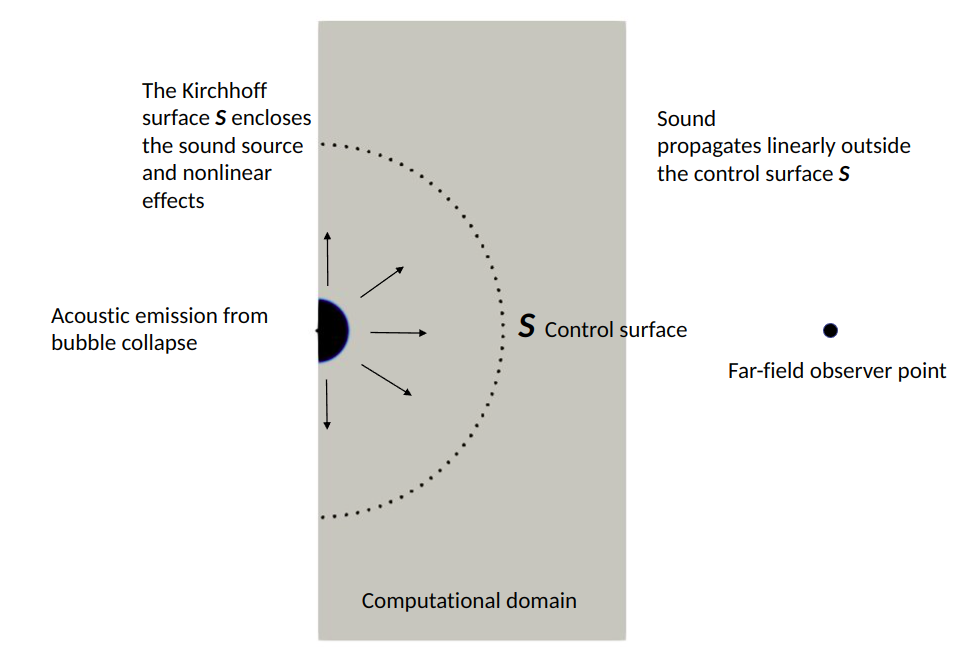
\includegraphics[scale=0.22]{images/schematic.png}
		\caption*{Schematic of far-field acoustic data computed from CFD solver using the Kirchhoff integral method.}
	\end{figure}
\end{frame}

\begin{frame}{Interpolation of pressure data}
	\begin{columns}
		\column{0.4\textwidth}
		\begin{figure}
			\centering
			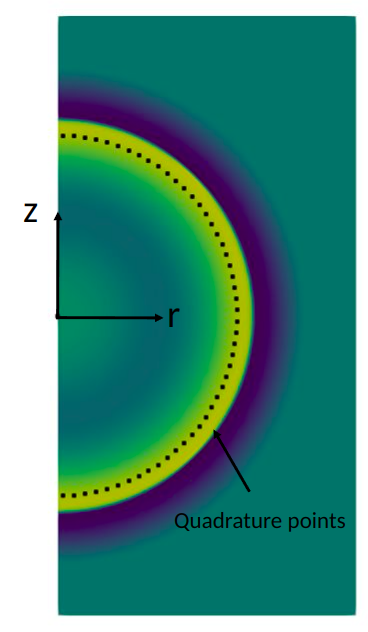
\includegraphics[scale=0.21]{images/arc.png}
			\caption*{The fourth-order WENO polynomial is used to interpolate the data at quadrature points and the four-point Lagrange polynomial is used to interpolate the data at the emission time.}
		\end{figure}
		\column{0.4\textwidth}
		\begin{figure}
			\centering
			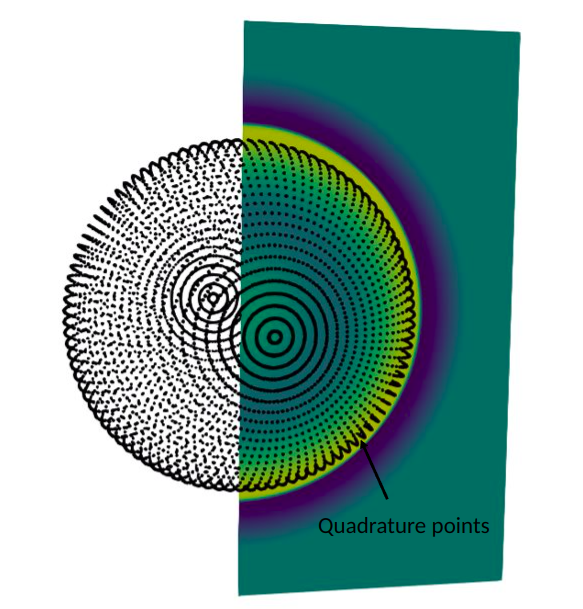
\includegraphics[scale=0.21]{images/sphere.png}
			\caption*{Using the axi-symmetry, the pressure data is copied along the azimuthal direction. We can use the Kirchhoff intergal on a spherical surface to compute the far-field pressure.}
		\end{figure}
	\end{columns}
\end{frame}

\begin{frame}{Kirchhoff integral on a sphere}
	\begin{itemize}
		\item We compute the Kirchhoff integral on a spherical surface 
		\begin{equation}
			\begin{split}
				p'(r, \theta, \phi,t) =  \frac{1}{4\pi}\int_{0}^{2\pi}\int_{0}^{\pi}\Big[  \frac{p'}{r'^{2}}&\frac{\partial r'}{\partial n} - \frac{1}{r'}\frac{\partial p'}{\partial n} + \frac{1}{c r'}\frac{\partial r'}{\partial n}\frac{\partial p'}{\partial \tau} \Big]_{\tau} R^2\sin\theta d\theta d \phi  
			\end{split} 
		\end{equation}
		\item The above integral is numerically computed using the mid-point rule 
		\begin{equation}
			\begin{split}
				p'(r, \theta, \phi,t) =  \frac{1}{4\pi} \sum_{i}^{N_{\theta}}\sum_{j}^{N_{\phi}}  \Big[  \frac{p'}{r'^{2}}&\frac{\partial r'}{\partial n} - \frac{1}{r'}\frac{\partial p'}{\partial n} + \frac{1}{c r'}\frac{\partial r'}{\partial n}\frac{\partial p'}{\partial \tau} \Big]_{\tau} R^2\sin\theta \Big|_{i, j} \Delta \theta \Delta \phi  
			\end{split} 
		\end{equation}
	\end{itemize}
\end{frame}

\begin{frame}{Kirchhoff solver: Convergence study}
	\begin{itemize}
		\item We solve the acoustic wave equation
		\begin{equation}
			\Bigg( \frac{1}{c_{0}^2}\frac{\partial{}^{2}}{\partial{t}^{2}}- \nabla{}^{2} \Bigg) p'(\mathbf{x}, t)  = -q(t)\delta(\mathbf{x}), 
		\end{equation}
		for a monopole source using the \textbf{Kirchhoff} method.
		\item And compare it with the exact solution $p'(\mathbf{x}, t) = -\frac{1}{4\pi} \frac{  q(t - \frac{r}{c_{0}}) }{r}$.
		\item We chose a monopole source
		\begin{equation}
			q(t) = 2(t - t0)f_{0}^{2}\exp( -f_{0}^2(t - t_{0})^{2}), 
		\end{equation}
		where $f_{0} = 100$ is the dominant frequency and $t_{0} = \frac{4}{f_{0}}$.
	\end{itemize}
\end{frame}

\begin{frame}{Kirchhoff solver: Convergence study}
	\begin{columns}
		\column{0.5\textwidth}
		\begin{figure}
			\centering
			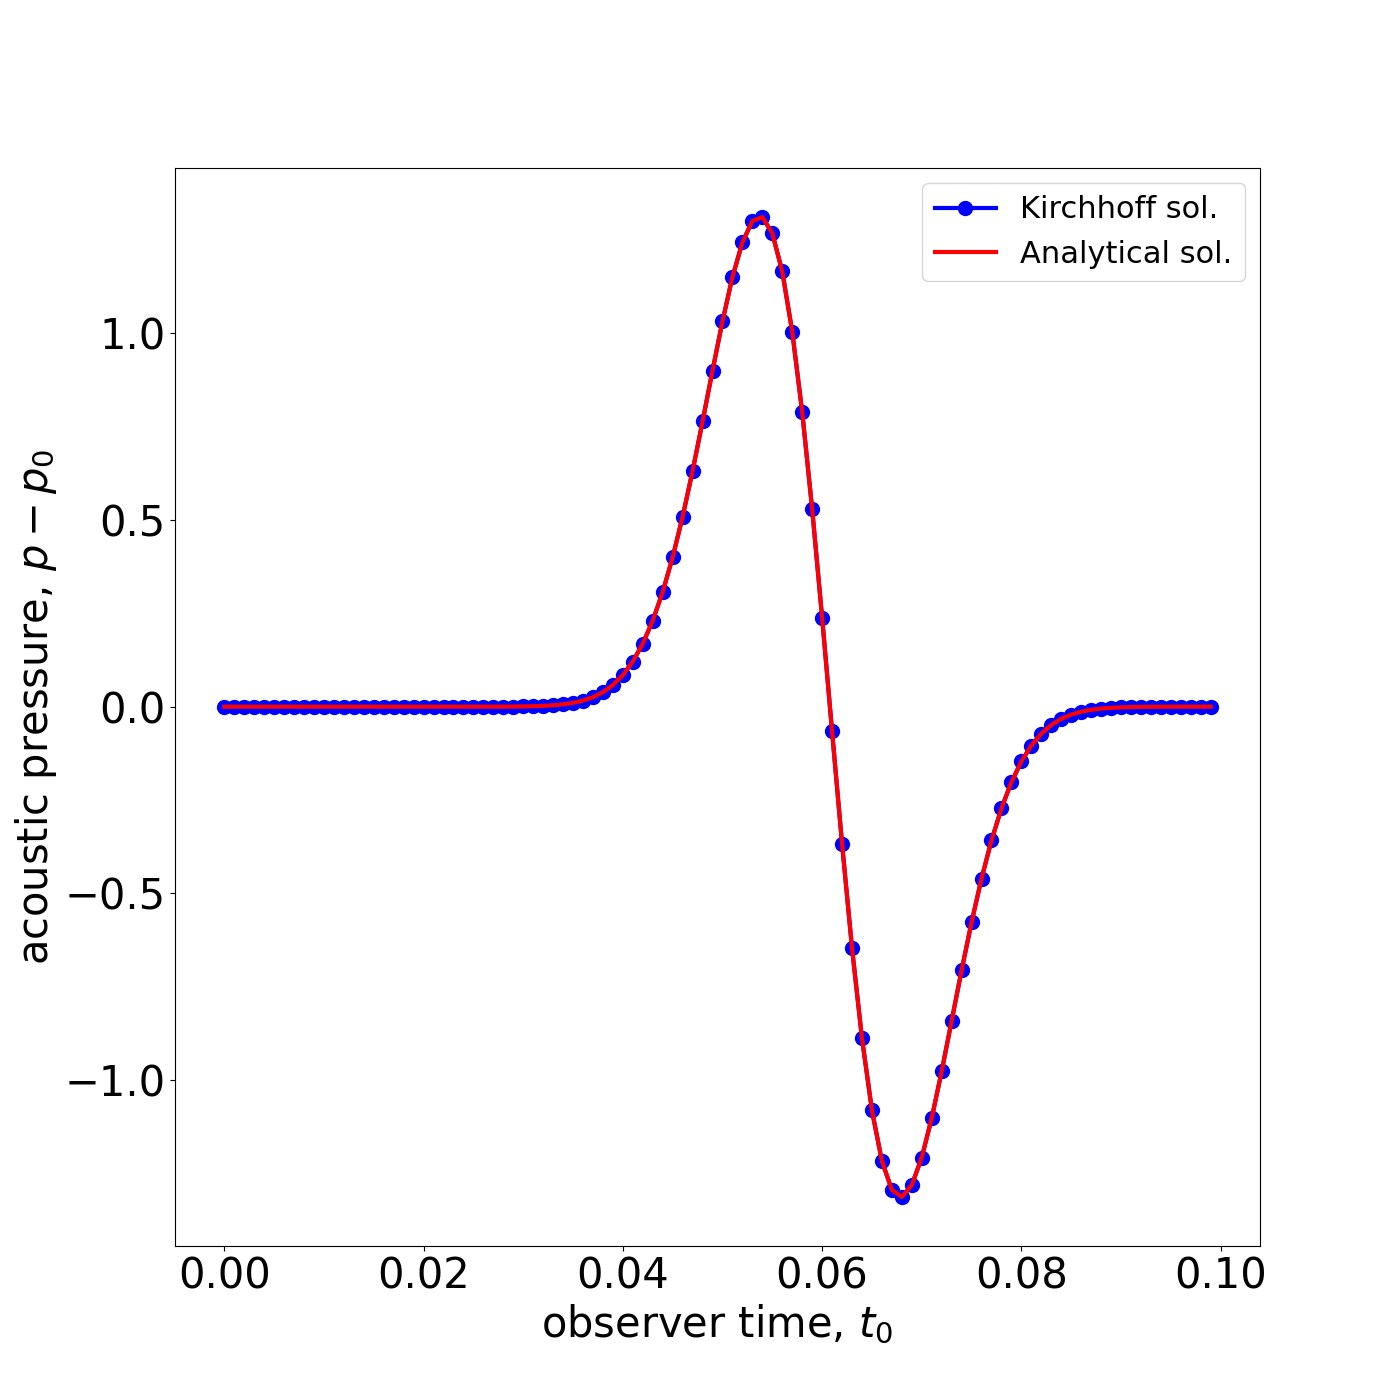
\includegraphics[scale=0.14]{images/Pressure.png}
			\caption*{Acoustic pressure computed using the Kirchhoff method and compared with the analytical solution at observer point $(x, y, z) = (3.0, 3.0, 3.0).$}
		\end{figure}
		\column{0.5\textwidth}
		\begin{figure}
			\centering
			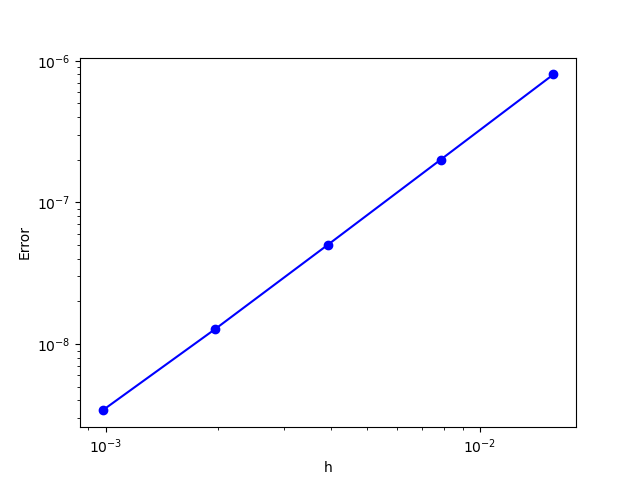
\includegraphics[scale=0.4]{images/convergence.png}
			\caption*{We have obtained second-order convergence for the Kirchhoff integral computed using the mid-point rule.}
		\end{figure}
	\end{columns}
\end{frame}


\begin{frame}{Results: Computation of acoustic waves from Rayleigh collapse}
							
	\begin{columns}
		\begin{column}{0.5\textwidth}
			\begin{itemize}
				\item air bubble in water
				\item Axi-symmetric domain $\Omega = [-10R,10R]\times[0,10R]$
				\item Radius of the bubble $R = 0.038 m$
				\item Discretization $500\times 250$ cells
				\item Boundary conditions:
				      \begin{itemize}
				      	\item top, bottom, left and right boundary $-$ transmissive 
				      \end{itemize}
			\end{itemize}
		\end{column}
																																			
		\begin{column}{0.5\textwidth}
			\begin{figure}
				\centering
				\begin{overpic}[scale=0.28,unit=1mm]{images/initial_condition.png}
					\put (10,81) {$\displaystyle \textcolor{white}{Water}$}
					\put (10,74) {\textcolor{white}{$\displaystyle \rho = 10^{3} kgm^{-3}$}}
					\put (10,67) {\textcolor{white}{$\displaystyle p = 1.0 MPa$ }}
					\put (10,60) {\textcolor{white}{$\displaystyle \gamma = 4.4$ }}															

					\put (5,37) {$\displaystyle \textcolor{white}{Air}$}
					\put (5,30) {\textcolor{white}{$\displaystyle \rho = 1.0 kgm^{-3}$}}
					\put (5,23) {\textcolor{white}{$\displaystyle p = 0.1 MPa$}}
					\put (5,16) {\textcolor{white}{$\displaystyle \gamma = 1.4$ }}
	

				\end{overpic}
				\caption*{Initial condition}
			\end{figure}
		\end{column}
														
	\end{columns}
\end{frame}

\begin{frame}{Results: Computation of acoustic waves from Rayleigh collapse}
							
	\begin{columns}
		\begin{column}{0.5\textwidth}
			\begin{itemize}
				\item The radius of the spherical Kirchhoff surface is $6R$
				\item The far-field observer point is at $(0, 9R)$ 
				\item The number of quadrature points $N_{\theta} = 500$ and $N_{\phi} = 1000$
				\item The speed of sound in the far-field acoustic medium is obtained from $\sqrt{\gamma(P + P_{\infty})/\rho}$	
			\end{itemize}
		\end{column}
																																			
		\begin{column}{0.32\textwidth}
			\begin{figure}
				\centering
				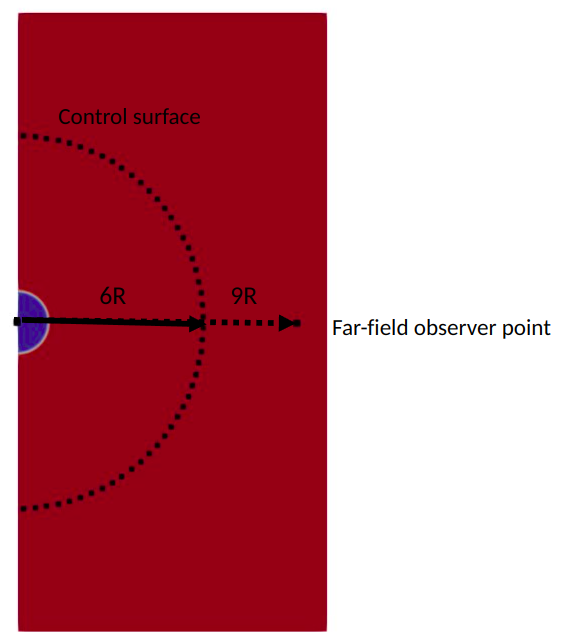
\includegraphics[scale=0.26]{images/schematic3.png}
				\caption*{Location of control surface and observer point}
			\end{figure}
		\end{column}
														
	\end{columns}
\end{frame}
\begin{frame}{Results: Computation of acoustic waves from Rayleigh collapse}
	\begin{columns}
		\begin{column}{.56\textwidth}
			\begin{figure}
				\centering
				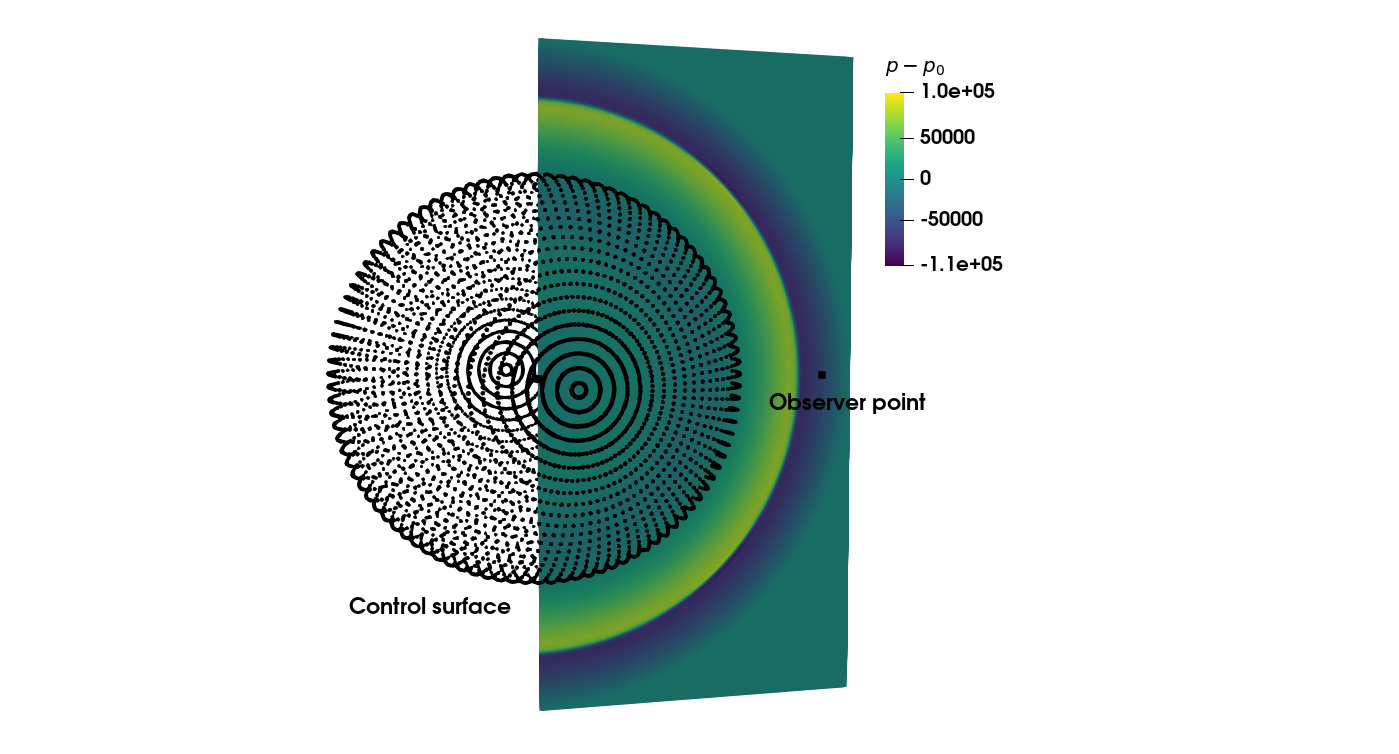
\includegraphics[scale=0.2]{images/acoustic_pressure.png}
				\caption*{Acoustic pressure emitted by bubble collapse reaches the observer point.}
			\end{figure}
		\end{column}
		\begin{column}{0.4\textwidth}
			\begin{figure}
				\centering
				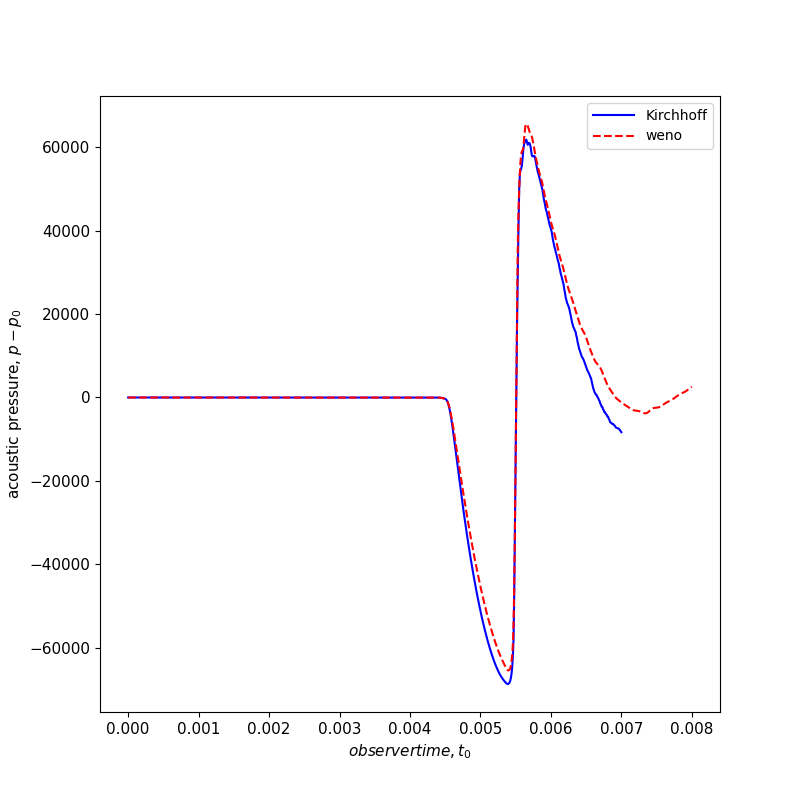
\includegraphics[scale=0.25]{images/structured_pressure.png}
				\caption*{Comparison of acoustic pressure at observer point from flow solver and Kirchhoff solver.}
			\end{figure}
		\end{column}
	\end{columns}	
\end{frame}
\begin{frame}{Conclusion and Future work}
	Conclusion:
	\begin{itemize}
		\item We have shown the second-order convergence for the numerical integration of the Kirchhoff integral using the mid-point rule for the acoustic waves emitted by the monopole.
		
	\end{itemize}
	Future work:
	\begin{itemize}
		\item Implement the fourth-order accurate axi-symmetric Kirchhoff solver.
		\item Compute far-field sound waves emitted by single and multiple bubble collapse process.
	\end{itemize}
\end{frame}

\begin{frame}[allowframebreaks]{Bibliography}
	\frametitle{Bibliography}
	\bibliographystyle{amsplain}
	\begin{thebibliography}{99}
		\bibitem{propeller} Duttweiler M. E., Brennen C. E. Surge instability on a cavitating propeller. Journal of Fluid Mechanics, 2002, 458: 133-152.
		\bibitem{Ffowcs} Ffowcs Williams, John E and David L Hawkings, Sound generation by turbulence and surfaces in arbitrary motion, Philosophical Transactions of the Royal Society of London. Series A, Mathematical and Physical Sciences 264, pp. 321-342, 1969.
		\bibitem{Farassat} F. Farassat and M.K. Myers, Extension of Kirchhoff's formula to radiation from moving surfaces, Journal of Sound and Vibration, 123, 451-460, 1988.
		\bibitem{Howe} Howe, MS, Theory of vortex sound. Cambridge university press 2003.
		\bibitem{Jamalludin} Jamaluddin, A., Ball, G., Turang, C., Leighton, T. The collapse of single bubbles and approximation of the far-field acoustic emissions for cavitation induced by shock wave lithotripsy. Journal of Fluid Mechanics, 677, 305-341. 2011.
	\end{thebibliography}
\end{frame}

\begin{frame}[standout]
	Thank you!
\end{frame}
\end{document}

%\bibitem{Jamaluddin} 
